\chapter{Méthode Formelle de description des architectures logiciel}
L'architecture des systèmes logiciel est très souvent décrite de façon informelle sous forme de diagrammes composés de boîtes et de lignes les reliant \cite{Gregory1995}. Cependant, bien que ces diagrammes soient interprétés en suivant des conventions définies, la nature informelle et imprécise de ses interprétations a de nombreuses limites. Nous pouvons citer à titre d'exemple l'ambiguïté dans la compréhension des architectures, la difficulté à analyser et tester automatiquement les modèles. 
\section{Description du langage  Z}
Développé à l'universite d'Oxford, le langage Z \cite{Gregory1995} est un langage formel. Ses racines mathématiques reposent essentiellement sur la logique de premeir ordre et la théorie des ensembles. La notation de Z utilise les connecteurs logiques standard (\land$, \lor$, \lnot, =>, etc.) et les opérations sur les ensembles (\in$, \cup$, \cap$, \subset$, etc.) tout en gardant leur signification originale. Pour décrire un système, les types (ou ensembles donnés) qui seront utilisés dans la spécification sont généralement listés au départ.

\subsection{Schéma de Z}
Dans la notation Z, les spécifications sont représentées par des boites compartimentées appelées \textit{schémas}. Un schéma décrit l'état d'un système ou les opérations possibles sur ce dernier. Un exemple de schéma est donné ci-après, il décrit l'enregistrement des passagers dans un avion. On considère pour cet exemple le type [PERSONNE] qui est l'ensemble des personnes identifiées de façon unique.

\begin{schema}{Avion}
capacite: \nat; aBord: \power_1~PERSONNE
\where
#aBord <= capacite
\znewpage
\end{schema}

La première partie de notre schéma contient les définitions de deux variables: capacité et aBord qui représentent respectivement la capacité de l'avion et le nombre de personnes à bord. La deuxième partie contient les contraintes sur ces variables. Dans notre cas, le nombre de personnes à bord de l'avion ne doit pas excéder la capacité de l'avion, ce qui est logique. 

\section{Formalisation d'une architecture de composants}
Pour représenter les architectures de logiciels à un niveau très abstrait, les composants sont souvent utilisés. Ces derniers interagissent entre eux pour faire fonctionner le système entier. Nous allons dans la suite nous intéresser à la formalisation d'une architecture de composants en utilisant \textbf{la notation Z}. Nous utiliserons pour se faire les travaux de \texttt{GREGORY D. ABOWD et al} dans \cite{Gregory1995}. 

Les trois éléments de base d'une architecture de composants sont: les composants, les connecteurs et les configurations des composants et connecteurs. 
\subsection{Les composants}
Les composants sont des unités fonctionnelles actives d'un système (voir figure \ref{fig:Z_component}). Ils accomplissent des tâches en faisant des traitements internes et des communications externes avec le reste du système. L'interaction entre les composants est définie explicitement comme une collection de points d'interaction ou ports. De façon intuitive, le port généralise la notion traditionnelle d'interface de modules. Dans les cas simples, un port peut représenter une procédure qui peut être appelée ou une variable qui peut être accédée dans l'interaction avec un autre composant. Un port peut tout aussi bien représenter, dans les cas plus complexes, une collection de procédures, un ensemble d’événements. Un composant, vu comme entité syntaxique, est un ensemble constitué de ports et d'une description de son traitement.
\begin{figure}[h!]
  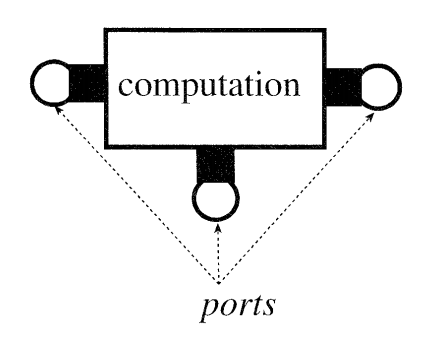
\includegraphics[scale=0.7]{images/composant_Z.png}
  \caption{Un composant}
  \label{fig:Z_component}
\end{figure}
La représentation formelle d'un composant avec la notation Z est donnée par la figure \ref{fig:Z_component_schema}.
\begin{figure}[h!]
  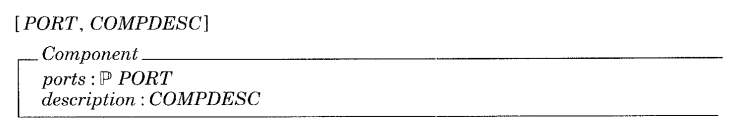
\includegraphics[scale=0.7]{images/Z_component_schema.png}
  \caption{Représentation d'un composant}
  \label{fig:Z_component_schema}
\end{figure}

\subsection{Les connecteurs}
Les connecteurs définissent les interactions entre composants (voir figure \ref{fig:Z_connector}). Ils permettent à des composants d'interagir en définissant la façon, le protocole de cette interaction. Tout comme les composants, les connecteurs sont des entités indépendantes. Un connecteur a une interface qui consiste en un ensemble de rôles. Chaque rôle définit le comportement que l'un des participants de l'interaction doit avoir. A titre d'exemple, un connecteur client-serveur a un rôle demandeur (le client) et un rôle fournisseur (le serveur); de même, un connecteur multicast aura un rôle annonceur et plusieurs rôles receveurs. Le comportement global d'un connecteur et des règles qu'il spécifie est défini de façon logique par un protocole. Par exemple, le protocole d'un connecteur client-serveur, nécessite que l'initialisation se fasse avant l'envoie de toute requête. Un connecteur architectural est alors modélisé comme une collection constituée de rôles et de la description de son protocole d'interaction comme décrit dans le schéma Connector.
\begin{figure}[h!]
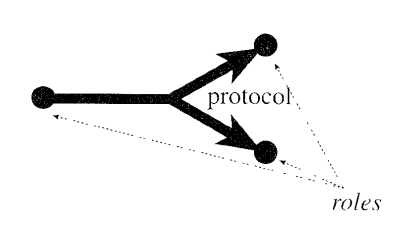
\includegraphics[scale=0.7]{images/connecteur_Z.png}
  \caption{Un connecteur}
  \label{fig:Z_connector}
\end{figure}
La représentation formelle d'un connecteur avec la notation Z est donnée par la figure \ref{fig:Z_connector_schema} suivante.
\begin{figure}[h!]
  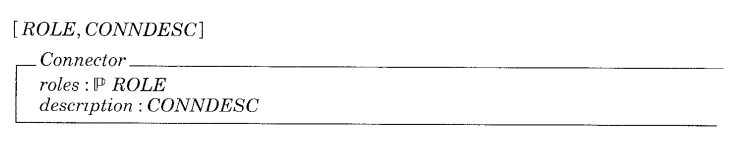
\includegraphics[scale=0.7]{images/Z_connector_schema.png}
  \caption{Représentation d'un connecteur}
  \label{fig:Z_connector_schema}
\end{figure}

\subsection{Les configurations}
Une configuration est une collection d'instances de composants qui interagissent au moyen d’instances de connecteurs (voir figure  \ref{fig:Z_configuration}). Les instances de composants et de connecteurs sont identifiés en nommant les éléments à partir de la classe syntaxique. Pour nommer les instances de composants et de connecteurs, nous introduisons deux ensembles: COMPNAME des noms possibles de composants et CONNNAME des noms de connecteurs. Ces ensembles sont aussi utilisés pour nommer les instances de ports associés à un composant ou de rôles associés à un connecteur.   Ainsi nous introduisons deux nouveaux types PortInst de tous les ports disponibles et RoleInst des instances de rôle illustré par la figure \ref{fig:Z_portInst_roleInst}.
\begin{figure}[h!]
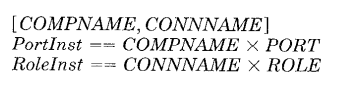
\includegraphics[scale=0.7, width=100mm]{images/Z_portInst_roleInst.png}
  \caption{PortInst et RoleInst}
  \label{fig:Z_portInst_roleInst}
\end{figure}

L'association entre les instances de composants et de connecteurs est modélisée par \texttt{des attachements} entre les rôles des connecteurs et les ports des composants.
\begin{figure}[h!]
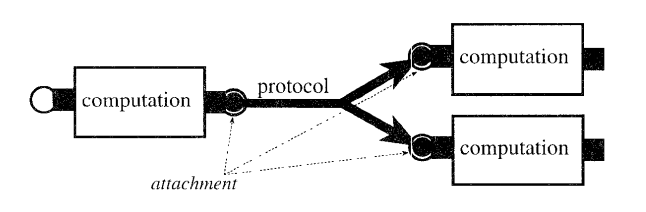
\includegraphics[scale=0.7]{images/configuration_Z.png}
  \caption{Une configuration}
  \label{fig:Z_configuration}
\end{figure}
La représentation formelle d'un connecteur avec la notation Z est donnée par la figure \ref{fig:Z_configuration_schema}.
\begin{figure}[h!]
  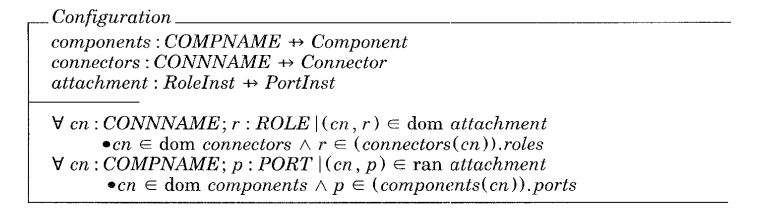
\includegraphics[scale=0.7]{images/Z_configuration_schema.png}
  \caption{Représentation d'une configuration}
  \label{fig:Z_configuration_schema}
\end{figure}

Le schéma \textsl{configuration} impose deux contraintes additionnelles (en dessous de la ligne de séparation) qui seront satisfaites par toutes les configurations. La première spécifie que toute instance de rôle dans l'attachement est un rôle pour un connecteur nommé dans la configuration. La seconde contrainte quant à elle assure que toutes les instances de ports décrites par la configuration doivent apparaître dans une instance actuelle de composants. Ces deux contraintes font respecter une portée lexicale sur les attachements au sein d'une configuration.
